% ARPEGOS:  Automatized Roleplaying-game Profile Extensible Generator Ontology based System %
% Author : Alejandro Muñoz Del Álamo %
% Copyright 2019 %

% Section 2.2: Planificación del Proyecto %
\section{Planificación del proyecto}
En este apartado se van a establecer el orden de las tareas que se 
deben realizar y la estimación del tiempo que se considera necesario 
para la elaboración de este proyecto. Finalmente se mostrará un 
análisis de la desviación temporal que indicará la diferencia entre los
tiempos estimados con los empleados realmente.

\subsection{Objetivo inicial}
El objetivo inicial de este proyecto era desarrollar una 
aplicación móvil para la generación y manipulación de información 
de personajes de juegos de rol, extensible a cualquier juego de rol 
cuya información esté almacenada en la aplicación.

\subsection{División del trabajo}
La estructura de desglose del trabajo está dispuesta a continuación: 

% Crear diagrama de división del trabajo
%\begin{figure}
%    \centering
%    \includegraphics[width=13cm]{Images/División_Trabajo.jpeg}
%    \caption{Estructura de desglose del trabajo}
%\end{figure}

\begin{itemize}
    \item \textbf{Planificación}: Inicialmente, se realiza una planificación \textit{grosso modo}, 
    que facilita una visión global de los hitos que se deben conseguir, y los 
    pasos adecuados para alcanzarlos.

    \item \textbf{Conocimientos}: Al inicio del proyecto, el equipo de desarrollo 
    de este proyecto no estaba relacionado con algunas de las herramientas que han sido 
    utilizadas. Por otra parte, otras herramientas sí eran conocidas por el equipo, pero 
    no con la profundidad que ha exigido el proyecto. Es precisamente esto lo que ha motivado 
    al equipo a recuperar la información que ya obtenía sobre las herramientas y ampliarla mediante 
    la búsqueda y lectura de documentación que pudiera beneficiar en el desarrollo.

    \item \textbf{Desarrollo}: Tras un breve período para ponerse al día con los 
    conocimientos básicos para comenzar el proceso de desarrollo, se realizarán los 
    diferentes \textit{sprints} con las siguientes tareas:
    
    \begin{itemize}
        \item \textbf{\textit{Planificación}}: Cada \textit{sprint} tendrá su 
        planificación específica seleccionando los requisitos \textit{necesarios} 
        para su desarrollo con el cliente. Como este proyecto \textit{no tiene un cliente claramente 
        definido, se ha entrevistado a \textbf{potenciales clientes}} de la aplicación 
        para poder conocer las necesidades que consideran oportunas como posibles 
        usuarios de la aplicación. Posteriormente, se procede a la planificación 
        del \textit{sprint} elaborando una lista de tareas que deben llevarse a 
        cabo para considerar que se ha finalizado el \textit{sprint} de manera
        satisfactoria.

        \item \textbf{\textit{Análisis}}
        \item \textbf{\textit{Diseño}}
        \item \textbf{\textit{Implementación}}: Se realizarán pruebas de funcionalidad 
        de manera simultánea a la codificación del proyecto, pudiendo comprobar que las 
        funciones finalizadas cumplen su función de forma correcta y completa, sin errores.

        \item \textbf{\textit{Documentación}}: Al finalizar cada \textit{sprint} se actualizará 
        la documentación del proyecto.
    \end{itemize}

    \item \textbf{Memoria}: Aunque la memoria se ha realizado de forma conjunta con el 
    proyecto desde su inicio, algunos aspectos como los manuales, han requerido que otros 
    aspectos del proyecto estuvieran finalizados para poder realizarse.

    \item \textbf{Presentación}: Elaboración de una presentación para la defensa del proyecto ante 
    el tribunal.
\end{itemize}

\subsection{Identificación de \textit{sprints} y estimación de tiempos}
El equipo de desarrollo procede, en este punto de la memoria, a describir 
las iteraciones que se han dado a lo largo de la elaboración del proyecto.

\begin{enumerate}
    
    \item \textbf{\textit{Sprint 0:} Planificación inicial}: Forman parte de esta 
    iteración tanto las reuniones con los clientes potenciales, como el estudio y 
    elección de las tecnologías a emplear.

    \item \textbf{\textit{Sprint 1:} Preparación del equipo}: Durante el primer \textit{sprint}
    se pondrá a punto el entorno de trabajo, instalando las aplicaciones necesarias para el 
    desarrollo. También se procederá a la instalación de aplicaciones que, no siendo necesarias, 
    serán de ayuda durante el proceso.

    \item \textbf{\textit{Sprint 2:} Creación de la ontología}: Este \textit{sprint} 
    es el más extenso de todos, debido a que abarca desde el esbozo inicial del modelo 
    conceptual de la ontología, que debe contener toda la información de un juego de rol, 
    hasta el momento en que ésta queda totalmente operativa.
    Como el sistema debe poder procesar otras ontologías además de la elaborada por el 
    equipo que lleva a cabo este proyecto, no se ha considerado finalizado el sprint 
    hasta que se han realizado todas las modificaciones necesarias, tanto en la lógica 
    de negocio de la aplicación como en la ontología, para que sea posible procesar y 
    disponer correctamente de toda la información de la ontología.

    \item \textbf{\textit{Sprint 3:} Creación de personajes}: El objetivo principal de 
    la aplicación se abordará en este \textit{sprint}, ya que requiere que la lógica de 
    negocio de la aplicación acceda a la ontología de un juego de rol, y extraiga información 
    de esta para mostrar un formulario de creación de personajes paso a paso, personalizado 
    para el juego de rol en cuestión, y que se genere un fichero con la información del personaje 
    que ha sido seleccionada por el usuario en el formulario.   

    \item \textbf{\textit{Sprint 4:} Visualización, modificación y eliminación de personaje}: La aplicación tiene que poder 
    mostrar la información del personaje creado previamente, y permitir al usuario editar parte de la misma si 
    así lo desea.

    \item \textbf{\textit{Sprint 5:} Validador de ontologías}: El proyecto dispondrá de una aplicación de consola 
    que permita comprobar a un desarrollador si la ontología del juego que está elaborando podría funcionar en la 
    aplicación principal del proyecto.

    \item \textbf{\textit{Sprint 6:} Cálculo de habilidades de personaje}: La aplicación podrá realizar 
    cálculos con la información almacenada en la hoja de personaje. Este campo se considera opcional, debido a que 
    al tener una fecha límite y un proceso complejo, es posible que no se pueda alcanzar este objetivo, el cual quedaría 
    pendiente como trabajo futuro.

    \item \textbf{\textit{Sprint 7:} Pruebas}: Se realizarán pruebas para comprobar que la aplicación cumple todos los 
    objetivos del proyecto.

    \item \textbf{\textit{Sprint 8:} Documentación}: La aplicación dispondrá de varios manuales que permitan a los 
    usuarios conocer sus funciones y la manera correcta de utilizarlas.

\end{enumerate}

\subsection{Resumen de la planificación del proyecto}
A continuación se muestra un resumen de la planificación previamente descrita desglosada según 
las actividades a realizar en un diagrama de Gantt.

\newpage

\begin{landscape}
    \begin{figure}[H]
        \centering
        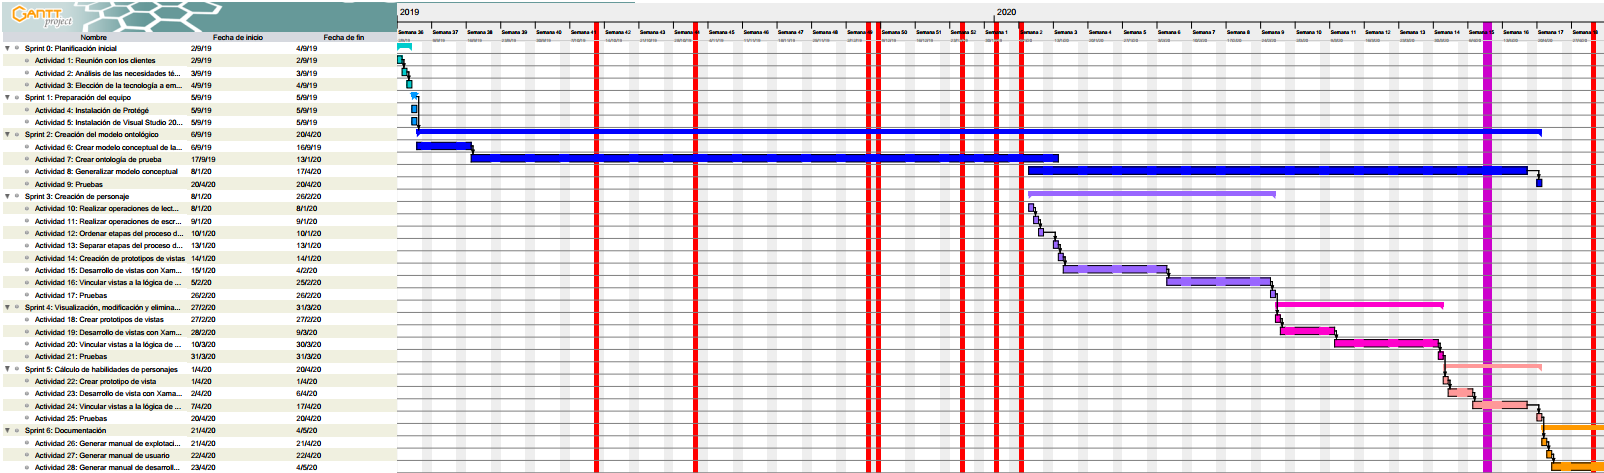
\includegraphics[scale=0.45]{Project_Planning/ARPEGOS_Gantt.png}
        \caption{Planificación del proyecto}
    \end{figure}
\end{landscape}
        

Los tiempos estimados han estado expuestos a imprevistos, ya fueran de tipo técnicos o tecnológicos:

\begin{itemize}
    \item \textit{Librería \textnormal{\textbf{dotNetRDF}} no permite trabajar con propiedades del formato \textnormal{\textbf{OWL}}}:
    La primera librería que el equipo encontró para poder trabajar con el formato \textit{RDF} fue \textbf{dotNetRDF}. El problema 
    sucedió cuando, una vez con el proyecto encaminado, resulta que la librería no es compatibles con las propiedades del formato \textit{OWL}, 
    de manera que no era posible realizar tuplas \textit{sujeto-predicado-objeto}, y por tanto, no es una librería compatible con la aplicación que 
    el equipo tiene como objetivo elaborar. Esto supuso un retraso de al menos un mes de trabajo para el equipo, ya que no sólo se había perdido 
    el tiempo dedicado en aprender a utilizar la librería, sino que era necesario buscar otra que permitiera realizar aquello que la primera no podía, 
    lo que podría hacer retroceder todo el proyecto, ya que de no encontrar una, habría que cambiar las herramientas base para el desarrollo.
    Después de buscar bastante, el equipo encontró la librería \textbf{RDFSharp}, que aún estando en desarrollo, sí es compatible con las propiedades 
    necesarias para realizar tuplas \textit{sujeto-predicado-objeto}, y por tanto, permite trabajar con el formato \textit{OWL}, siendo así compatible 
    con el producto final.

    \item \textit{Error en el SO causa error en repositorios del proyecto}: Durante una de las actualizaciones del proyecto, el sistema operativo del 
    ordenador que realizaba la actualización, causó la corrupción de gran parte de los ficheros del proyecto, resultando afectados los repositorios local 
    y remoto del proyecto. El equipo entonces hizo uso de una copia de seguridad almacenada en un dispositivo externo, para recuperar la mayor cantidad 
    de trabajo posible, pero al no estar actualizado completamente, fue necesario invertir entre 7 y 8 horas para recuperar el trabajo perdido.
\end{itemize}

% Introducir tablas de horas estimadas y reales %








